\documentclass[conference,letterpaper]{IEEEtran}
% Four technical pages and a reference-only fifth page. No margin/font shrinking.
\usepackage[T1]{fontenc}
\usepackage{newtxtext,newtxmath}
\usepackage{amsmath,booktabs,array,tabularx}
\usepackage{graphicx,tikz}
\usetikzlibrary{arrows.meta,positioning,calc}
\usepackage{cite}
\usepackage[hidelinks]{hyperref}
\usepackage{microtype}
\newcommand{\epl}{EP-L2}
\newcommand{\base}{B16}
\newcommand{\unif}{U-WB16}
\newcolumntype{L}[1]{>{\raggedright\arraybackslash}p{#1}}
% Real, fixed-height layout reservations. They intentionally contain no fake data.
\newcommand{\resultpanel}[4]{\fbox{\begin{minipage}[c][#2][c]{\dimexpr#1-2\fboxsep-2\fboxrule\relax}\centering
\small\textbf{#3}\par\medskip
\footnotesize MEASUREMENTS PENDING\par\medskip
\parbox{.91\linewidth}{\centering\footnotesize #4}
\end{minipage}}}
\hypersetup{pdftitle={EP-L2: Elastic Payload Storage for In-Place Writeback in GPU L2 Caches},pdfauthor={EP-L2 project; author information pending},pdfsubject={EN-v2: revised structure, real figure reservations, verified references; no empirical results}}
\hyphenation{write-back micro-ar-chi-tec-ture in-di-rec-tion}
\begin{document}
\title{EP-L2: Elastic Payload Storage for\\In-Place Writeback in GPU L2 Caches}
\author{\IEEEauthorblockN{Author information to be completed}\IEEEauthorblockA{English working draft EN-v2 --- not for submission}}
\maketitle
\begin{abstract}
In a fixed-partition GPU L2, a dirty victim may need to move from resident storage to a writeback buffer even though only its consumer has changed. The copy consumes bank service, while static role quotas prevent idle capacity from being borrowed. Elastic Payload L2 (EP-L2) separates resident-tag visibility, physical data ownership, and writeback ordering. A dirty victim becomes writeback-staged in its original slot; the incoming resident receives a distinct, bank-compatible slot. The design retains the reference's payload capacity and bank-service budget, eliminating resident-to-writeback copying without adding resident tags or miss-tracking entries. We specify the ownership protocol and a matched evaluation that separates copy elimination, relief of staging-capacity pressure, and application performance. Independently qualified application measurements and physical implementation results remain pending; this working draft makes no empirical speedup, area, or energy claim.
\end{abstract}
\begin{IEEEkeywords}
GPU, L2 cache, writeback, tag--data decoupling, resource sharing
\end{IEEEkeywords}

\section{Introduction}
A cache line's visibility, data, and transaction state need not have the same lifetime. On a dirty eviction, the old resident tag can become reusable before the lower memory system accepts the data. Same-address ordering may persist even after that transfer. A design must preserve the data and ordering obligations without unnecessarily retaining the original tag or moving data merely to change their role.

We study an L2 with fixed quotas for resident, bypass-return, and writeback-buffer (WBUF) payloads. Its banked reference copies a dirty victim into WBUF before reusing the resident slot. The copy requires a source read and destination write; sending the staged line requires another read. A larger WBUF can relieve a quota limit but does not remove the copy. Conversely, fewer copy operations need not improve execution time if another resource determines progress.

The design insight is to transfer ownership rather than location. In \epl{}, the dirty payload remains in place, while an independently allocated slot receives the incoming resident line. All roles share the same total data capacity, but the resident-tag count stays fixed. The mechanism can thus reduce internal movement and expose idle slots to transient consumers; these are distinct potential benefits.

Tag--data indirection and storage unification have been explored previously. V-Way decouples tag and data placement~\cite{vway}; unified GPU local memory reallocates capacity among registers, cache, and scratchpad~\cite{unified}; in-cache MSHR storage and MiCache reuse cache storage for pending-request information~\cite{farkas,micache}. Our focus is instead the \emph{resident-to-writeback data lifetime}: retaining dirty data in place while separately releasing tag visibility and address-ordering state. This transition requires evaluating both data-service demand and access to otherwise idle capacity.

This paper presents the in-place writeback protocol and its bounded resource model, then organizes evaluation around three questions: which bank operations disappear, whether static staging capacity actually blocks progress, and whether useful L2 service improves application execution. Optional victim-retention and read-only paths are scoped separately; they are not prerequisites for the primary writeback comparison.

\section{EP-L2 Design}
\subsection{One-Slice Organization and Matched Reference}
Figure~\ref{fig:organization} places the payload pool beside the distinct lookup, request-tracking, and ordering structures. The primary reference, \base{} (\texttt{B16\_BANKED}), has 1024 resident, 128 bypass-return, and 16 WBUF payload slots. \unif{} (\texttt{U\_WB16}) dynamically shares the same 1168 slots. Each slot is 128 B, with four 32-B sectors. Both modes provision four banks of 292 slots and at most one line-sized operation per bank per \emph{physical} GPU cycle. Both also provision a common 128-B copy latch outside the allocatable pool.

\begin{figure*}[t]
\centering
\begin{minipage}[t]{.49\textwidth}
\centering\small\textbf{(a) Logical organization of one L2 slice}\par\smallskip
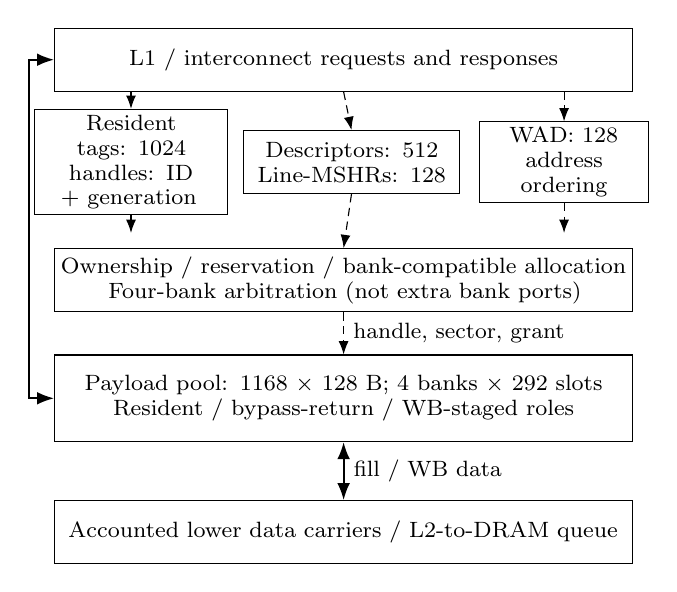
\begin{tikzpicture}[x=1mm,y=1mm,>=Latex,font=\fontsize{8}{9}\selectfont,
box/.style={draw,align=center,inner sep=2pt,minimum height=8mm},
ctl/.style={->,densely dashed,line width=.4pt},data/.style={<->,line width=.7pt}]
\node[box,text width=72mm] (in) at (40,53) {L1 / interconnect requests and responses};
\node[box,text width=23mm] (tag) at (13,40) {Resident tags: 1024\\handles: ID + generation};
\node[box,text width=26mm] (req) at (41,40) {Descriptors: 512\\Line-MSHRs: 128};
\node[box,text width=20mm] (wad) at (68,40) {WAD: 128\\address ordering};
\node[box,text width=72mm] (ctrl) at (40,25) {Ownership / reservation / bank-compatible allocation\\Four-bank arbitration (not extra bank ports)};
\node[box,text width=72mm,minimum height=11mm] (pool) at (40,10) {Payload pool: 1168 $\times$ 128 B; 4 banks $\times$ 292 slots\\Resident / bypass-return / WB-staged roles};
\node[box,text width=72mm] (low) at (40,-7) {Accounted lower data carriers / L2-to-DRAM queue};
\draw[ctl] (in.south)--(req.north);
\draw[ctl] (13,49)--(tag.north);\draw[ctl] (68,49)--(wad.north);
\draw[ctl] (tag.south)--(13,31);\draw[ctl] (req.south)--(ctrl.north);\draw[ctl] (wad.south)--(68,31);
\draw[ctl] (ctrl.south)--node[right]{handle, sector, grant} (pool.north);
\draw[data] (pool.south)--node[right]{fill / WB data} (low.north);
\draw[data] (in.west)--(0,53)--(0,10)--(pool.west);

\end{tikzpicture}
\end{minipage}\hfill
\begin{minipage}[t]{.49\textwidth}
\centering\small\textbf{(b) Copy removal and separate release events}\par\smallskip
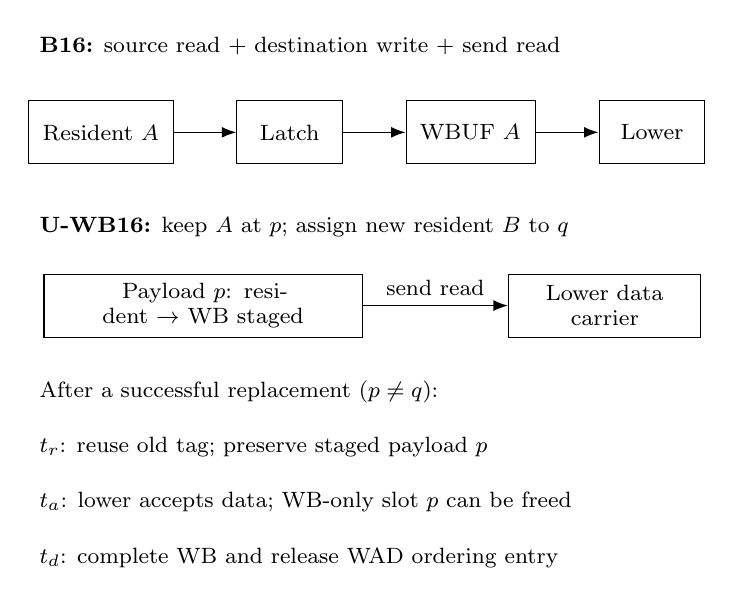
\begin{tikzpicture}[x=1mm,y=1mm,>=Latex,font=\fontsize{8}{9}\selectfont,
box/.style={draw,align=center,inner sep=2pt,minimum height=8mm},arr/.style={->,line width=.5pt}]
\node[anchor=west] at (0,55) {\textbf{B16:} source read $+$ destination write $+$ send read};
\node[box,text width=17mm] (a) at (9,44) {Resident $A$};
\node[box,text width=12mm] (l) at (33,44) {Latch};
\node[box,text width=15mm] (w) at (56,44) {WBUF $A$};
\node[box,text width=12mm] (d) at (79,44) {Lower};
\draw[arr] (a)--(l);\draw[arr] (l)--(w);\draw[arr] (w)--(d);
\node[anchor=west] at (0,32) {\textbf{U-WB16:} keep $A$ at $p$; assign new resident $B$ to $q$};
\node[box,text width=39mm] (p) at (22,22) {Payload $p$: resident $\to$ WB staged};
\node[box,text width=23mm] (lo) at (73,22) {Lower data carrier};
\draw[arr] (p)--node[above]{send read} (lo);
\node[anchor=west] at (0,11) {After a successful replacement ($p\ne q$):};
\node[anchor=west] at (0,4) {$t_r$: reuse old tag; preserve staged payload $p$};
\node[anchor=west] at (0,-3) {$t_a$: lower accepts data; WB-only slot $p$ can be freed};
\node[anchor=west] at (0,-10) {$t_d$: complete WB and release WAD ordering entry};
\end{tikzpicture}
\end{minipage}
\caption{Declared WB-only design, not a physical floorplan or a measured cycle schedule. Dashed links denote control dependencies; solid links denote data movement. B16 uses fixed 1024/128/16 role quotas over the same banks; U-WB16 shares those slots. Both retain a 128-B copy latch outside the pool. Optional TVD/RO consumers are not drawn as extra data arrays.}
\label{fig:organization}
\end{figure*}


A tag names a payload by \{slot identifier, generation\}. Each slot has one authoritative owner; valid/pending sector masks and pins protect its consumers. The initial design retains the resident bank class,
\begin{equation}
 \operatorname{bank}(p)=p\bmod4=\operatorname{tag\_index}\bmod4.
\label{eq:bank}
\end{equation}
A globally free slot is therefore not necessarily a legal landing slot for a particular replacement. The fixed 1024 resident tags remain the lookup-capacity limit, even when resident data use previously nonresident slots.

\subsection{Reservation, In-Place Transition, and Release}
Before replacing a dirty line, the controller reserves the WAD entry, required issue resources, and a legal data destination. In \base{}, the old data are read from the resident bank and written through the latch to WBUF. Only after that copy is safe can the original resident slot be reused. WBUF subsequently supplies a bank read for the lower send.

In \unif{}, a dirty line $A$ retains payload $p$ and changes role to \texttt{WB\_STAGED}. A different slot $q$ is reserved for the new resident $B$; its tag points to $q$, not $p$. This removes resident-to-WBUF copying, but retains the send read, lower-queue occupancy, and receiving data carrier. Failed reservation leaves the old tag, owner, and pending state unchanged. Accepted requests always have a reserved return location.

At committed replacement time $t_r$, the tag can be reused; the staged payload survives until actual lower data acceptance $t_a$. The writeback address directory (WAD) maintains ordering until real completion $t_d$. Merely enqueueing a software pointer does not establish that the lower path owns the data. The receiving carrier must be accounted for before the local staging slot is released. A late event for $A$ uses its transaction/handle identity and cannot modify $B$ through a reused tag index.

Pins survive bank reads and response backpressure. Partial-sector readiness does not make a whole line valid, and old generations cannot access reused storage. The WB drain path does not require admission of a new resident miss. This prevents that local allocation cycle, assuming eventual bank and lower-system service; it is not a whole-GPU deadlock proof.

\subsection{Optional Consumers and Implementation Cost}
TVD retains victim payloads without resident tags, using a shared WAD/TVD budget of 128 address entries and one additional lookup cycle after a tag miss. Valid-sector reads can be served in place; clean writes/atomics require promotion, while dirty writes/atomics wait for writeback completion. Retained data remain explicitly owned. The RO extension separately controls pending-tag detachment and Line-MSHR bypass under a complete-commandlist, line-granular read-only oracle. Detached fills complete original consumers without reinstalling replaced tags. Both extensions are OFF in the primary \base{}/\unif{} experiment and receive no extra payload array or descriptor pool.

Primary payload storage is 146 KiB/slice, or 9.125 MiB over 64 slices; common latches add 8 KiB/chip. An identifier needs $P=\lceil\log_2 1168\rceil=11$ bits. Explicit tag handles cost $1024(P+G)$ bits for generation width $G$; up to 128 WB handles add $128(P+G)$ bits plus state and packet binding. Shared baseline fields are not counted again as pooling overhead. Generation width, pin bounds, allocation selection, arbitration, rollback state, and lookup ports require a concrete hardware mapping. Symbolic verification versions are not payload RAM or automatically hardware fields. Equal storage and bank budgets do not establish equal area or frequency; matched RTL, SRAM macros, and timing/power measurements remain necessary.

\begin{figure*}[t]
\centering
\resultpanel{.486\textwidth}{40mm}{(a) Application performance}{Five fixed workloads: convolutionSeparable, FWT, CFD, vectorAdd, sad.\\Paired cycles and $C_B/C_U$; include slowdowns.}
\hfill
\resultpanel{.486\textwidth}{40mm}{(b) Measured WB and copy work}{Source reads, destination writes, send reads, and completed WB totals.\\Common denominator and units stated per panel.}
\caption{Reserved main-result area. The two panels will use the same current-qualified binary and matched inputs. No bars, values, reference line, or mean have been fabricated; blank space is intentional.}
\label{fig:mainresults}
\end{figure*}

\section{Evaluation Methodology}
\subsection{Controlled Comparison and Workloads}
The implementation uses Accel-Sim's SASS flow and the GPGPU-Sim performance-model lineage~\cite{accelsim,gpgpusim}. These citations identify the tools; their hardware-correlation results do not validate our modified L2. The same independently qualified repaired binary must execute both modes with identical complete traces, non-mode configurations, timing scope, and termination rules. Table~\ref{tab:configuration} lists the declared research configuration, not undocumented commercial-GPU internals.

\begin{table}[t]
\caption{Matched evaluation configuration (per slice unless stated).}
\label{tab:configuration}\centering\footnotesize
\begin{tabularx}{\columnwidth}{@{}L{.42\columnwidth}X@{}}
\toprule
Resource & Setting \\
\midrule
Resident / total payload & 1024 tags / 1168 slots (146 KiB) \\
Line / sectors / banks & 128 B / $4\times32$ B / $4\times292$ slots \\
Bank service / copy latch & 1 op/bank/physical cycle / 128 B \\
Descriptors / Line-MSHRs & 512 / 128; at most 32 requesters/address \\
WAD / L2-to-DRAM queue & 128 / 128 entries \\
Chip / memory channels & 64 slices / 32 channels \\
DRAM / scheduler / return & 850 MHz / 128 / 192 entries per channel \\
L1 (fixed) & 64 KiB/core; 4 banks; 20-cycle setting \\
WBUF8 sensitivity & 1160 slots, 145 KiB; $4\times290$ bankslots \\
\bottomrule
\end{tabularx}
\end{table}

The development set is convolutionSeparable, FWT\_7\_21, cfd\_097k, vectorAdd\_4M, and sad; sad is the low-pressure negative control. Btree and dwt2d are reserved for validation after policy selection, with scan scheduled separately. Slowdowns remain in the result set. A five-workload geometric mean is computed only after every pair satisfies the common criteria, rather than averaging a favorable completed subset.

\subsection{Correctness and Timing Qualification}
Directed tests exercise actual cache/partition paths, not only detached helper models. They cover nonzero host-memcpy offsets, at most one bank grant per physical cycle, valid host-prefill payload identity, generation reuse, sector returns, response backpressure, and distinct WB data-acceptance/completion events. Native tag-ordering timestamps must not alter bank-service time. Host prefill rejects dirty, pinned, pending, or nonquiescent state before mutation.

Complete numerical payloads are unavailable in the SASS traces. The supported checks are therefore ownership, symbolic sector versions, requester/transaction identity, and final resource drain, not full numerical application correctness. Source/binary/configuration/trace identities and current independent acceptance accompany every result. Normal exit or a historical certificate cannot override later qualification withdrawal.

\section{Results and Causal Analysis}
\noindent\textbf{Result status.} No currently qualified application pair is available for this revision. Figures~\ref{fig:mainresults}--\ref{fig:controls} are fixed-size reservations for actual measurements, not plotted results. Earlier invalidated runs are excluded. The following specifies how each panel will support or reject a claim; findings will replace this text after acceptance.

\subsection{End-to-End Performance and Copy Work}
Figure~\ref{fig:mainresults}(a) is reserved for the full five-workload \base{}/\unif{} comparison. With matching instruction counts and timing scope, speedup is $S=C_{\base}/C_{\unif}$. Pairwise cycles accompany the figure, and negative controls and regressions remain visible.

For one otherwise equivalent completed WB episode, the specified reference performs three logical staging/send bank operations, whereas the in-place path performs the send read only. This is a protocol count, not a 3$\times$ speedup. Actual runs may evict different numbers of lines; Fig.~\ref{fig:mainresults}(b) therefore reports measured copy/send operations and WB totals in both modes. Retry attempts are not new logical operations, and a reduction per episode must not be substituted for the measured application total.

\begin{figure*}[t]
\centering
\resultpanel{.319\textwidth}{46mm}{(a) Capacity and ordering}{Staged/reserved occupancy; WB-data-full and pool/landing waits.\\WAD pressure shown separately.}
\hfill
\resultpanel{.319\textwidth}{46mm}{(b) Useful bank service}{Logical operations; physical grants and grant-limit check; waiting per operation.\\Not a subtraction from elapsed cycles.}
\hfill
\resultpanel{.319\textwidth}{46mm}{(c) Downstream pressure}{Matched lower/DRAM bytes and queue/service evidence.\\Separate lower acceptance from WB completion.}
\caption{Reserved causal-analysis area. These three panels distinguish staging capacity, bank service, and pressure transferred downstream. Metrics with different units must not share an unlabeled scale. The future data determine the conclusion, not the panel titles.}
\label{fig:causal}
\end{figure*}

\subsection{Capacity Pressure, Service, and Downstream Effects}
A nonzero borrowing counter does not demonstrate a capacity benefit. Figure~\ref{fig:causal}(a) relates WB-data-full waits to staged/reserved occupancy, pool-full or bank-compatible landing failures, and separately recorded WAD pressure. A capacity claim needs binding static quota pressure \emph{and} useful allocation from otherwise inaccessible slots. An idle bypass partition may supply headroom in this workload set, but does not establish the best static partition.

Figure~\ref{fig:causal}(b) separates logical operations, physical bank grants, and waiting. Summed per-operation waits are not elapsed GPU cycles and cannot be directly subtracted from application time. Fig.~\ref{fig:causal}(c) tests whether improved admission merely transfers pressure to the lower queue, scheduler, or DRAM. WB-data release at lower acceptance and WAD release at completion must remain distinguishable. Together, these panels connect copy/capacity changes to useful service rather than only to counters that happen to decrease.

\begin{figure}[t]
\centering
\resultpanel{\columnwidth}{36mm}{Strong control / sensitivity}{Equal-total-capacity static repartition and/or the planned WBUF8 sensitivity.\\Select only after the stated scientific preconditions.}
\caption{Reserved control panel. A fixed repartition tests whether an allocation chosen in advance suffices; a copy-service diagnostic tests a different cause. This slot is not a claim that either experiment has run.}
\label{fig:controls}
\end{figure}

\subsection{Strong Controls and Cost Sensitivity}
When capacity sharing contributes, Fig.~\ref{fig:controls} uses an equal-1168-slot static repartition, such as 1024 resident/112 bypass/32 WBUF. Its reduced bypass quota is an explicit cost. An independently qualified equal-copy-service diagnostic may be needed when copy elimination could explain the difference. The already planned WBUF8 sensitivity checks a second budget; these comparisons do not add free metadata or bank ports.

If local service improves without end-to-end benefit, a representative case crosses baseline/mechanism with original/one justified downstream-headroom setting. This four-point interaction test differs from simply showing that faster memory helps both modes. Ideal WB-capacity, metadata, and read-hit diagnostics require a separate same-binary baseline and remain optimistic diagnostics, not implemented \epl{} performance. Optional TVD/RO results enter only after their own qualification; the reserved panels do not authorize new experiments.

The final interpretation must also include added control latency and implementation cost. Equal data bytes are not equal area, and fewer bank accesses alone do not establish energy savings. Macro energy, arbitration/selection, wiring, leakage, and execution duration need compatible implementation inputs. No physical PPA number is available in this revision.

\section{Related Work and Scope}
\textbf{Flexible storage organization.} V-Way increases tag capacity relative to data and uses indirection for demand-based associativity~\cite{vway}. Tag-Split Cache instead changes data-storage granularity while retaining coarse request granularity~\cite{tsc}. \epl{} fixes resident tags and line/sector sizes, targeting cross-role payload lifetimes rather than either form of spatial packing.

\textbf{Storage reused for transient state.} In-cache MSHR designs reuse cache storage for pending-load information, subject to placement and port constraints~\cite{farkas}. MiCache shares FPGA storage between cache lines and MSHR subentries, converting MSHR entries to cache entries on response~\cite{micache}. \epl{} instead retains existing dirty \emph{data} during resident-to-WB transition, with request metadata and WAD separately bounded.

\textbf{Other resource and access policies.} Gebhart \emph{et al.} repartition SM-local registers/cache/scratchpad storage at kernel boundaries; their evaluated cache is write-through~\cite{unified}. DL-MSHR links slots to adapt primary/secondary-miss capacity; its slots can also carry write-miss data~\cite{dlmshr}. MRPB reorders and bypasses requests before GPU L1 access~\cite{mrpb}, whereas victim caching retains displaced lines for reuse~\cite{victim}. These address related resource limits but are not direct implementations of the WB-only comparison. Potential combinations require measurement rather than assumed additive benefit.

\section{Conclusion}
\epl{} transfers dirty-payload ownership without relocating the data, while separating resident visibility and WB ordering. Its architectural effects are fewer copy operations and more flexible access to a fixed payload budget. Their workload value must be established through matched performance, true capacity pressure, service, and cost evidence. The reserved result panels make that remaining evaluation explicit without presenting unmeasured benefits.

% Keep the optional fifth page reference-only. No technical appendix on that page.
\clearpage
% Generated by IEEEtran.bst, version: 1.14 (2015/08/26)
\begin{thebibliography}{10}
\providecommand{\url}[1]{#1}
\csname url@samestyle\endcsname
\providecommand{\newblock}{\relax}
\providecommand{\bibinfo}[2]{#2}
\providecommand{\BIBentrySTDinterwordspacing}{\spaceskip=0pt\relax}
\providecommand{\BIBentryALTinterwordstretchfactor}{4}
\providecommand{\BIBentryALTinterwordspacing}{\spaceskip=\fontdimen2\font plus
\BIBentryALTinterwordstretchfactor\fontdimen3\font minus
  \fontdimen4\font\relax}
\providecommand{\BIBforeignlanguage}[2]{{%
\expandafter\ifx\csname l@#1\endcsname\relax
\typeout{** WARNING: IEEEtran.bst: No hyphenation pattern has been}%
\typeout{** loaded for the language `#1'. Using the pattern for}%
\typeout{** the default language instead.}%
\else
\language=\csname l@#1\endcsname
\fi
#2}}
\providecommand{\BIBdecl}{\relax}
\BIBdecl

\bibitem{vway}
M.~K. Qureshi, D.~Thompson, and Y.~N. Patt, ``The {V-Way} cache: Demand-based
  associativity via global replacement,'' in \emph{Proceedings of the 32nd
  Annual International Symposium on Computer Architecture (ISCA)}, 2005, pp.
  544--555.

\bibitem{unified}
M.~Gebhart, S.~W. Keckler, B.~Khailany, R.~Krashinsky, and W.~J. Dally,
  ``Unifying primary cache, scratch, and register file memories in a throughput
  processor,'' in \emph{Proceedings of the 45th Annual IEEE/ACM International
  Symposium on Microarchitecture (MICRO)}, 2012, pp. 96--106.

\bibitem{farkas}
K.~I. Farkas and N.~P. Jouppi, ``Complexity/performance tradeoffs with
  non-blocking loads,'' Digital Equipment Corporation, Western Research
  Laboratory, Research Report 94/3, Mar. 1994.

\bibitem{micache}
S.~Xu, S.~Lu, Z.~Shao, X.~Liao, and H.~Jin, ``{MiCache}: An {MSHR}-inclusive
  non-blocking cache design for {FPGAs},'' in \emph{Proceedings of the 2024
  ACM/SIGDA International Symposium on Field Programmable Gate Arrays (FPGA)},
  2024, pp. 22--32.

\bibitem{accelsim}
M.~Khairy, Z.~Shen, T.~M. Aamodt, and T.~G. Rogers, ``{Accel-Sim}: An
  extensible simulation framework for validated {GPU} modeling,'' in
  \emph{Proceedings of the 47th Annual International Symposium on Computer
  Architecture (ISCA)}, 2020, pp. 473--486.

\bibitem{gpgpusim}
A.~Bakhoda, G.~L. Yuan, W.~W.~L. Fung, H.~Wong, and T.~M. Aamodt, ``Analyzing
  {CUDA} workloads using a detailed {GPU} simulator,'' in \emph{Proceedings of
  the IEEE International Symposium on Performance Analysis of Systems and
  Software (ISPASS)}, 2009, pp. 163--174.

\bibitem{tsc}
L.~Li, A.~B. Hayes, S.~L. Song, and E.~Z. Zhang, ``Tag-split cache for
  efficient {GPGPU} cache utilization,'' in \emph{Proceedings of the 2016
  International Conference on Supercomputing (ICS)}, 2016, pp. 43:1--43:12.

\bibitem{dlmshr}
Y.~Gu and L.~Chen, ``Dynamically linked {MSHRs} for adaptive miss handling in
  {GPUs},'' in \emph{Proceedings of the International Conference on
  Supercomputing (ICS)}, 2019, pp. 510--521.

\bibitem{mrpb}
W.~Jia, K.~A. Shaw, and M.~Martonosi, ``{MRPB}: Memory request prioritization
  for massively parallel processors,'' in \emph{Proceedings of the 20th IEEE
  International Symposium on High Performance Computer Architecture (HPCA)},
  2014, pp. 272--283.

\bibitem{victim}
N.~P. Jouppi, ``Improving direct-mapped cache performance by the addition of a
  small fully-associative cache and prefetch buffers,'' in \emph{Proceedings of
  the 17th Annual International Symposium on Computer Architecture (ISCA)},
  1990, pp. 364--373.

\end{thebibliography}
\end{document}
